\documentclass[]{article}
\usepackage[utf8]{inputenc}
\usepackage[ngerman]{babel}
\usepackage[T1]{fontenc}
\usepackage{%
	ngerman,
	ae,
	times,  %% hier kann man die Schriftart einstellen
	graphicx,
	url,
	scrlayer-scrpage,
	lastpage,
	mathtools,
	geometry,
	multicol,
	cancel,
	xcolor,
	nicematrix,
	xfrac,
	tikz,
	pgfplots,
	amsmath,
	colortbl,
	centernot,
	dsfont,
	textgreek,
	icomma,
	pdfpages}
\usepackage[thinlines]{easybmat}
\usetikzlibrary{datavisualization}
\usetikzlibrary{datavisualization.formats.functions}
\usetikzlibrary{intersections}
\pgfplotsset{compat=1.17}
\newcommand{\del}[1]{\cancel{~#1~}}
\NiceMatrixOptions{ last-col,code-for-last-col = \color{blue}\scriptstyle,light-syntax}
\newlength\dlf
\newcommand\alignedhighlight[3]{
  % #1 = color
  % #2 = before alignment
  % #3 = after alignment
  &
  \begingroup
  \settowidth\dlf{$\displaystyle #2$}
  \addtolength\dlf{\fboxsep+\fboxrule}
  \hspace{-\dlf}
  \fcolorbox{#1}{#1}{$\displaystyle #2 #3$}
  \endgroup
}
\newcommand{\reference}[1]{ \text{\small{\textcolor{blue}{(#1)}}} }

\newcommand{\topic}{Elektrotechnisch-phys. Grundlagen}
\newcommand{\subtopic}{Praktikum: Versuch 3}
\newcommand{\authors}{Nils Helming}

%Head and Footnotes
\setlength{\headheight}{2.1\baselineskip} %baselineskip = minimum distance bbetween the bottom of one line to another.
\geometry{bottom = 3cm}
\setlength{\headsep}{\baselineskip}
\ihead[\topic\hrule]{\topic\hrule}
\chead[\subtopic\\~]{\subtopic\\~}
\ohead[\authors\\~]{\authors\\~}
\ifoot[~]{~}
\cfoot[~]{~}
\ofoot[Seite \thepage~von \pageref{LastPage}]{Seite \thepage~von \pageref{LastPage}}

%Paragraph spacings
\setlength{\parindent}{0em} %em = with of an 'M'
\setlength{\parskip}{1ex} %ex = height of an 'x'

\newcommand{\V}{\lor}
\newcommand{\A}{\land}
\newcommand{\T}[1]{\overline{#1}}
\newcommand{\eq}{\Leftrightarrow}
\newcommand{\rarr}{\Rightarrow}
\newcommand{\red}[1]{\textcolor{red}{#1}}

\newcommand{\unit}[1]{\text{#1}}
\newcommand{\fracunit}[2]{\frac{\unit{#1}}{\unit{#2}}}
\newcommand{\textsq}[1]{\ensuremath{\text{#1}^2}}
\newcommand{\textpow}[2]{\ensuremath{\text{#1}^{#2}}}
\newcommand{\tdot}{\ensuremath{\cdot}}


\begin{document}
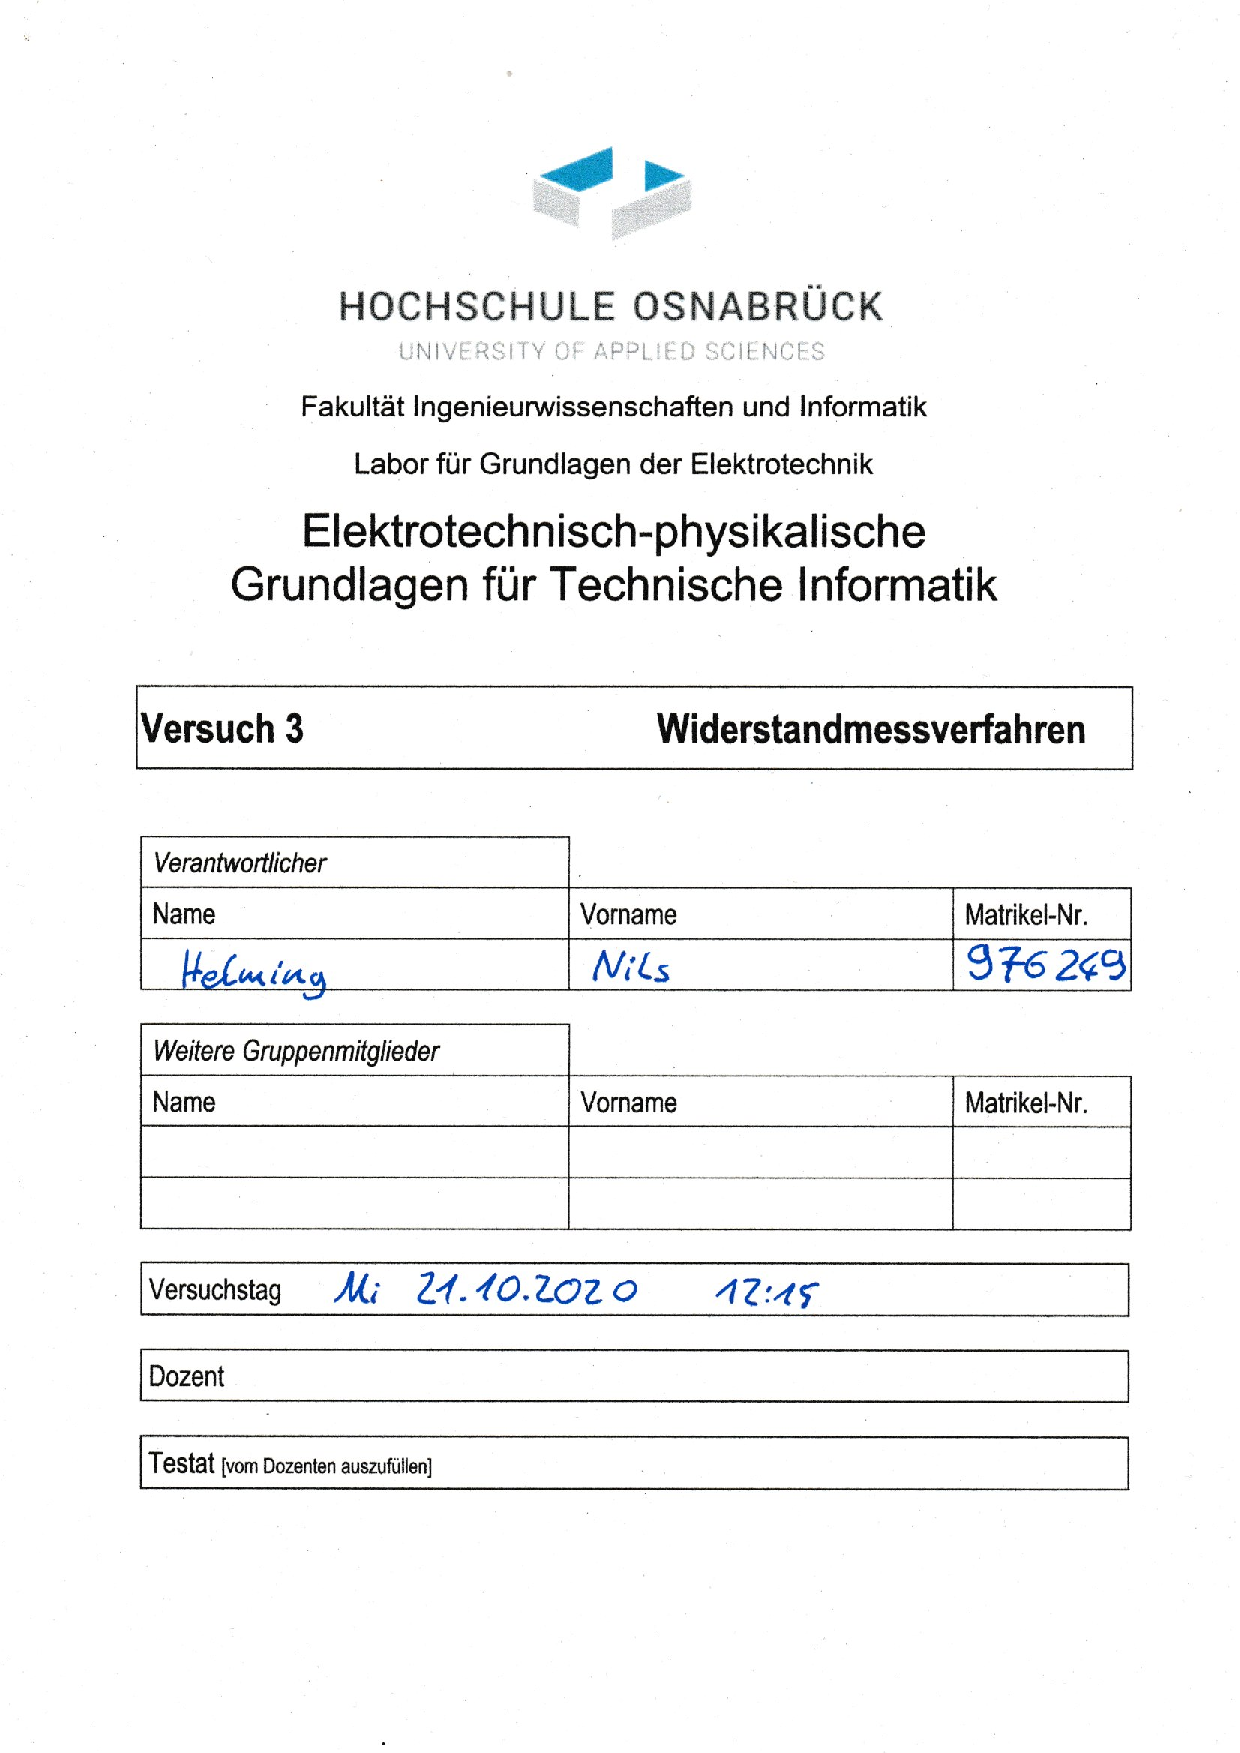
\includepdf[pages=-]{Deckblatt.pdf}
\section*{Aufgabe 1:}
	In diesem Versuch sollten Widerstände ($2,7\unit{\textOmega}$ und $10\unit{k\textOmega}$) mittels Strom- und Spannungsfehlerschaltungen gemessen werden. Dabei sollte klar werden, wie sich die Messgeräte auf die Messungen auswirken.
\subsection*{(a) \normalfont Widerstände unter Vernachlässigung der Messgeräte}
	Wenn die Messwerte für Strom und Spannung ohne Berücksichtigung auf die Innenwiderstände der jeweiligen Messgeräte berechnet werden, kommen wir auf folgende Widerstandswerte:

	\textbf{(1)} Stromfehlerschaltung mit $2,7\unit{\textOmega}$ Widerstand:\\
	Es wurde ein Strom von $500\unit{mA}$ und eine Spannung von $1,36\unit{V}$ gemessen.\\ Somit würden wir einen Widerstand von $R = \frac{U}{I} = \frac{1,36\unit{V}}{500\unit{mA}} = 2,72\unit{\textOmega}$ erwarten.

	\textbf{(2)} Stromfehlerschaltung mit $10\unit{k\textOmega}$ Widerstand:\\
	Hier haben sich Messungen von $4,75\unit{V}$ und $0,5\unit{mA}$ ergeben.\\ Damit hätten wir einen Widerstand von $R = \frac{U}{I} = \frac{4,75\unit{V}}{0,5\unit{mA}} = 9,5\unit{k\textOmega}$ gemessen.

	\textbf{(3)} Spannungsfehlerschaltung mit $2,7\unit{\textOmega}$ Widerstand:\\
	Hier wurden $1,78\unit{V}$ Spannung bei $500\unit{mA}$ festgestellt.\\ Der zu erwartende Widerstand wäre damit $R = \frac{U}{I} = \frac{1,78\unit{V}}{500\unit{mA}} = 3,56\unit{\textOmega}$.

	\textbf{(4)} Spannungsfehlerschaltung mit $10\unit{k\textOmega}$ Widerstand:\\
	In diesem Fall sind $5,2\unit{V}$ Spannung bei $0,5\unit{mA}$ festgestellt worden.\\ Der gemessene Widerstand ist also $R = \frac{U}{I} = \frac{5,2\unit{V}}{0,5\unit{mA}} = 10,4\unit{k\textOmega}$.

\subsection*{(b) \normalfont Widerstände bei Berücksichtigung der jeweiligen zuzüglichen Innenwiderstände}
	Unter Berücksichtigung der zusätzlichen Innenwiderstände des jeweilig relevanten Messgeräts ergeben sich diese Widerstände:

	In der Stromfehlerschaltung bestimmt das Amperemeter nicht nur den Strom durch den Widerstand $R_x$, sondern auch den Strom durch das Voltmeter. Also haben wir in (a) den gesamten Widerstand $R_{ges}$ über das Voltmeter und den gesuchten Widerstand bestimmt. Da das Voltmeter parallel zu $R_x$ steht ist dessen Widerstand $R_{iV}$ in folgender Relation zu den übrigen:
	\begin{align*}
		&&\frac{1}{R_{ges}} &= \frac{1}{R_{iV}}+\frac{1}{R_x}&&\\
		\eq&& \frac{1}{R_x} &= \frac{1}{R_{ges}}-\frac{1}{R_{iV}}&&\\
		\eq&& \frac{1}{R_x} &= \frac{R_{iV}}{R_{ges}\cdot R_{iV}}-\frac{R_{ges}}{R_{iV} \cdot R_{ges}}&&\\
		\eq&& \frac{1}{R_x} &= \frac{R_{iV}-R_{ges}}{R_{iV} \cdot R_{ges}}&&\\
		\eq&& R_x &= \frac{R_{iV} \cdot R_{ges}}{R_{iV}-R_{ges}}&&\\
	\end{align*}

	\textbf{(1)} Stromfehlerschaltung mit $R_x = 2,7\unit{\textOmega}$:\\
	Hier hat sich $R_{ges} = 2,72\unit{\textOmega}$ ergeben. Der wärend dem Versuch bestimmte Innenwiderstand war $R_{iV} = 60\unit{k\textOmega}$. Aus der obigen Gleichung folgt dann:
	\begin{align*}
		&&R_x &= \frac{R_{iV} \cdot R_{ges}}{R_{iV}-R_{ges}}&&\\
		&& &= \frac{60\unit{k\textOmega} \cdot 2,72\unit{\textOmega}}{60\unit{k\textOmega} - 2,72\unit{\textOmega}}&&\\
		&& &\approx 2,72\unit{\textOmega}&&\\
	\end{align*}

	\textbf{(2)} Stromfehlerschaltung mit $R_x = 10\unit{k\textOmega}$:\\
	Hier hat sich $R_{ges} = 9,5\unit{k\textOmega}$ ergeben. Der wärend dem Versuch bestimmte Innenwiderstand war $R_{iV} = 200\unit{k\textOmega}$. Aus der obigen Gleichung folgt dann:
	\begin{align*}
		&&R_x &= \frac{R_{iV} \cdot R_{ges}}{R_{iV}-R_{ges}}&&\\
		&& &= \frac{200\unit{k\textOmega} \cdot 9,5\unit{k\textOmega}}{200\unit{k\textOmega} - 9,5\unit{k\textOmega}}&&\\
		&& &\approx 9974\unit{\textOmega}&&\\
	\end{align*}

	In der Spannungsfehlerschaltung bestimmt das Voltmeter nicht nur den Spannungsabfall durch den Widerstand $R_x$, sondern zusätzlich den Spannungsabfall an dem Amperemeter. Da wir in (a) den gesamten Widerstand $R_{ges}$ über den gesuchten Widerstand $R_x$ und das Amperemeter gemessen haben, liegen $R_x$ und der Innenwiderstand $R_{iA}$ des Amperemeters in Reihe. Also gilt:
	\begin{align*}
		&&R_{ges} &= R_{iA} + R_x &&\\
		\eq&&R_x &= R_{ges} - R_{iA} &&\\
	\end{align*}

	\textbf{(3)} Spannungsfehlerschaltung mit $R_x = 2,7\unit{\textOmega}$:\\
	Hier hat sich $R_{ges} = 3,56\unit{\textOmega}$ ergeben. Der wärend dem Versuch bestimmte Innenwiderstand war $R_{iA} = 0,9\unit{\textOmega}$. Aus der obigen Gleichung folgt dann:
	\begin{align*}
		&&R_x &= R_{ges} - R_{iA} &&\\
		&& &= 3,56\unit{\textOmega} - 0,9\unit{\textOmega}&&\\
		&& &= 2,66\unit{\textOmega}&&\\
	\end{align*}

	\textbf{(4)} Spannungsfehlerschaltung mit $R_x = 10\unit{k\textOmega}$:\\
	Hier hat sich $R_{ges} = 10,4\unit{k\textOmega}$ ergeben. Der wärend dem Versuch bestimmte Innenwiderstand war $R_{iA} = 480,4\unit{\textOmega}$. Aus der obigen Gleichung folgt dann:
	\begin{align*}
		&&R_x &= R_{ges} - R_{iA} &&\\
		&& &= 10,4\unit{k\textOmega} - 480,4\unit{\textOmega}&&\\
		&& &\approx 9,9\unit{k\textOmega}&&\\
	\end{align*}

\section*{Aufgabe 2:}
\begin{samepage}
	Es wurde ein NTC mit immer steigenden Strömen betrieben. Dieser war zunächst in einem Glasgefäß von der Umluft abgeschlossen. Es wurden die dabei resultierenden Ströme und Spannungsabfälle notiert. Zuletzt wurde bei dem höchst angelegten Strom der NTC aus dem Gefäß entnommen und in der Luft bewegt.

	Zunächst sollten die Messwerte aus dem Messprotokoll Grafisch dargestellt werden.
	\begin{center}
		\begin{tikzpicture}
			\begin{axis}[
				width=0.95\textwidth,
				height=0.6\textwidth,
				legend pos=south east,
				xmin=0,
				xmax=22.5,
				ymin=0,
				ymax=12.5,
				extra x ticks={0},
				extra y ticks={0},
				axis lines=center,
				xlabel={$I$ in mA},
				ylabel={$U(I)$ in V},
				xlabel style={right},
				ylabel style={above},
				smooth,
				% no markers,
			]
				\addplot[color=black,mark=*, only marks] coordinates {
					( 0.47,  2.97)
					( 0.89,  5.40)
					( 1.81,  8.95)
					( 2.73, 10.64)
					( 3.66, 11.39)
					( 4.70, 11.63)
					( 5.65, 11.60)
					( 7.62, 11.28)
					( 9.65, 10.86)
					(13.51,  9.95)
					(17.43,  9.16)
					(21.40,  8.51)
				};
				\addlegendentry{Messpunkte}
				\draw[fill=blue, opacity = 0.1] (axis cs:0,0) rectangle (axis cs:4.7,12);
				%Der folgende Plot ist nur für die Legende da.
				\addplot[line width=10pt, color=blue, opacity = 0.1, no marks] coordinates {(-1,-1)};
				\addlegendentry{Fremderwärmung}
				\draw[fill=red, opacity = 0.1] (axis cs:4.7,0) rectangle (axis cs:22.5,12);
				%Der folgende Plot ist nur für die Legende da.
				\addplot[line width=10pt, color=red, opacity = 0.1, no marks] coordinates {(-1,-1)};
				\addlegendentry{Eigenerwärmung}
				% \addplot[thick, color=blue, no marks] coordinates {
				% 	( 0.47,  2.97)
				% 	( 0.89,  5.40)
				% 	( 1.81,  8.95)
				% 	( 2.73, 10.64)
				% };
				% \addlegendentry{Fremderwärmung}
				% \addplot[thick, color=red, no marks] coordinates {
				% 	( 2.73, 10.64)
				% 	( 3.66, 11.39)
				% 	( 4.70, 11.63)
				% 	( 5.65, 11.60)
				% 	( 7.62, 11.28)
				% 	( 9.65, 10.86)
				% 	(13.51,  9.95)
				% 	(17.43,  9.16)
				% 	(21.40,  8.51)
				% };
				% \addlegendentry{Eigenerwärmung}
			\end{axis}
		\end{tikzpicture}
	\end{center}

	Der Widerstand erhöht sich wärend Luftbewegung, da (dem Namen nach: Negative Temperature Coefficient) der NTC negative Temperatur-Koeffizienten (z.B. $\alpha_{20}$) hat. Also der Widerstand sinkt, wenn die Temperatur steigt. Oder andersherum: Der Widerstand steigt, sofern die Temperatur sinkt. Duch die Bewegung kann der NTC - welcher zu diesem Zeitpunkt in Eigenerwärmung war - mehr Hitze an die umliegende Luft verlieren, die Temperatur des NTC sinkt also. Und damit steigt der Widerstand des NTC.
\end{samepage}

\newpage
\section*{Aufgabe 3:}
	Hier sollte ein Widerstand mittels Spannungsabgleich bestimmt werden. Dafür wurde eine Schleifdrahtmessbrücke zusammen mit einem bekannten Widerstand ($R_4 = 1\unit{k\textOmega}$) verwendet. Die Position der Schleifdrahtmessbrücke zum Zeitpunkt des Abgleichs wurde zusammen mit der Gesamtlänge notiert.

	Da in dieser Aufgabe eine Schleifdrahtmessbrücke verwendet wurde, um den Spannungsabgleich zu erreichen, können wir folgende Gleichung anwenden:
	\begin{align*}
		&&R_x &= R_4 \cdot \frac{x}{l-x} &&\\
	\end{align*}
	In unserem Fall wurde ein Widerstand $R_4 = 1\unit{k\textOmega}$ vorgegeben und die Gesamtlänge der Messbrücke betrag $l = 100\unit{cm}$. Der Ausgleich wurde bei $x=54,6\unit{cm}$ erreicht. Damit ergibt sich:
	\begin{align*}
		&&R_x &= R_4 \cdot \frac{x}{l-x} &&\\
		&& &= 1\unit{k\textOmega} \cdot \frac{54,6\unit{cm}}{100\unit{cm}-54,6\unit{cm}} &&\\
		&& &\approx 1,2\unit{k\textOmega}&&\\
	\end{align*}

\newpage
\section*{Aufgabe 4:}
	Es sollten die spezifischen Widerstände von drei verschiedenen Metallstäben ($d = 4\unit{mm}$) bestimmt werden. Dafür wurde mit einer Vierleiteranordnung Strom und Spannung über einen Großteil der Metalle gemessen.

	Die Querschnittsfläche der drei Stäbe beträgt $A = \pi \cdot (4\unit{mm})^2 = 50,3\unit{\textsq{mm}}$ und der Abstand zwischen den Messspitzen ist $l = 0,25\unit{m}$. Aus der folgenden Gleichung lassen sich dann die spezifischen Widerstände der Metalle bestimmen:
	\begin{align*}
		&&R &= \frac{\rho \cdot l}{A} &&\\
		\eq&& \rho &= \frac{R \cdot A}{l} &\text{mit }U &= I \cdot R\text{:}\\
		\eq&& &= \frac{U \cdot A}{I \cdot l} &&\\
		\\%XXXXXX Aluminium XXXXXXX
		\text{\textbf{(1)} Aluminiumlegierung: }&& \rho_A &= \frac{2,295\unit{mV} \cdot 50,3\unit{\textsq{mm}}}{10\unit{A} \cdot 0,25\unit{m}} &&\\
		&& &\approx 46,2\fracunit{m\textOmega \textsq{mm}}{m} &&\\
		&& &= 46,2 * 10^{-3}\fracunit{\textOmega \textsq{mm}}{m}&&\\
		&& &= 46,2 * 10^{-7}\unit{\textOmega cm}&&\\
		\\%XXXXXX Kupferlegierung XXXXXXX
		\text{\textbf{(2)} Kupferlegierung: }&& \rho_K &= \frac{0,856\unit{mV} \cdot 50,3\unit{\textsq{mm}}}{10\unit{A} \cdot 0,25\unit{m}} &&\\
		&& &\approx 17,2\fracunit{m\textOmega \textsq{mm}}{m} &&\\
		&& &= 17,2 * 10^{-3}\fracunit{\textOmega \textsq{mm}}{m}&&\\
		&& &= 17,2 * 10^{-7}\unit{\textOmega cm}&&\\
		\\%XXXXXX Messing XXXXXXX
		\text{\textbf{(3)} Messing: }&& \rho_M &= \frac{3,607\unit{mV} \cdot 50,3\unit{\textsq{mm}}}{10\unit{A} \cdot 0,25\unit{m}} &&\\
		&& &\approx 72,6\fracunit{m\textOmega \textsq{mm}}{m} &&\\
		&& &= 72,6 * 10^{-3}\fracunit{\textOmega \textsq{mm}}{m}&&\\
		&& &= 72,6 * 10^{-7}\unit{\textOmega cm}&&\\
	\end{align*}




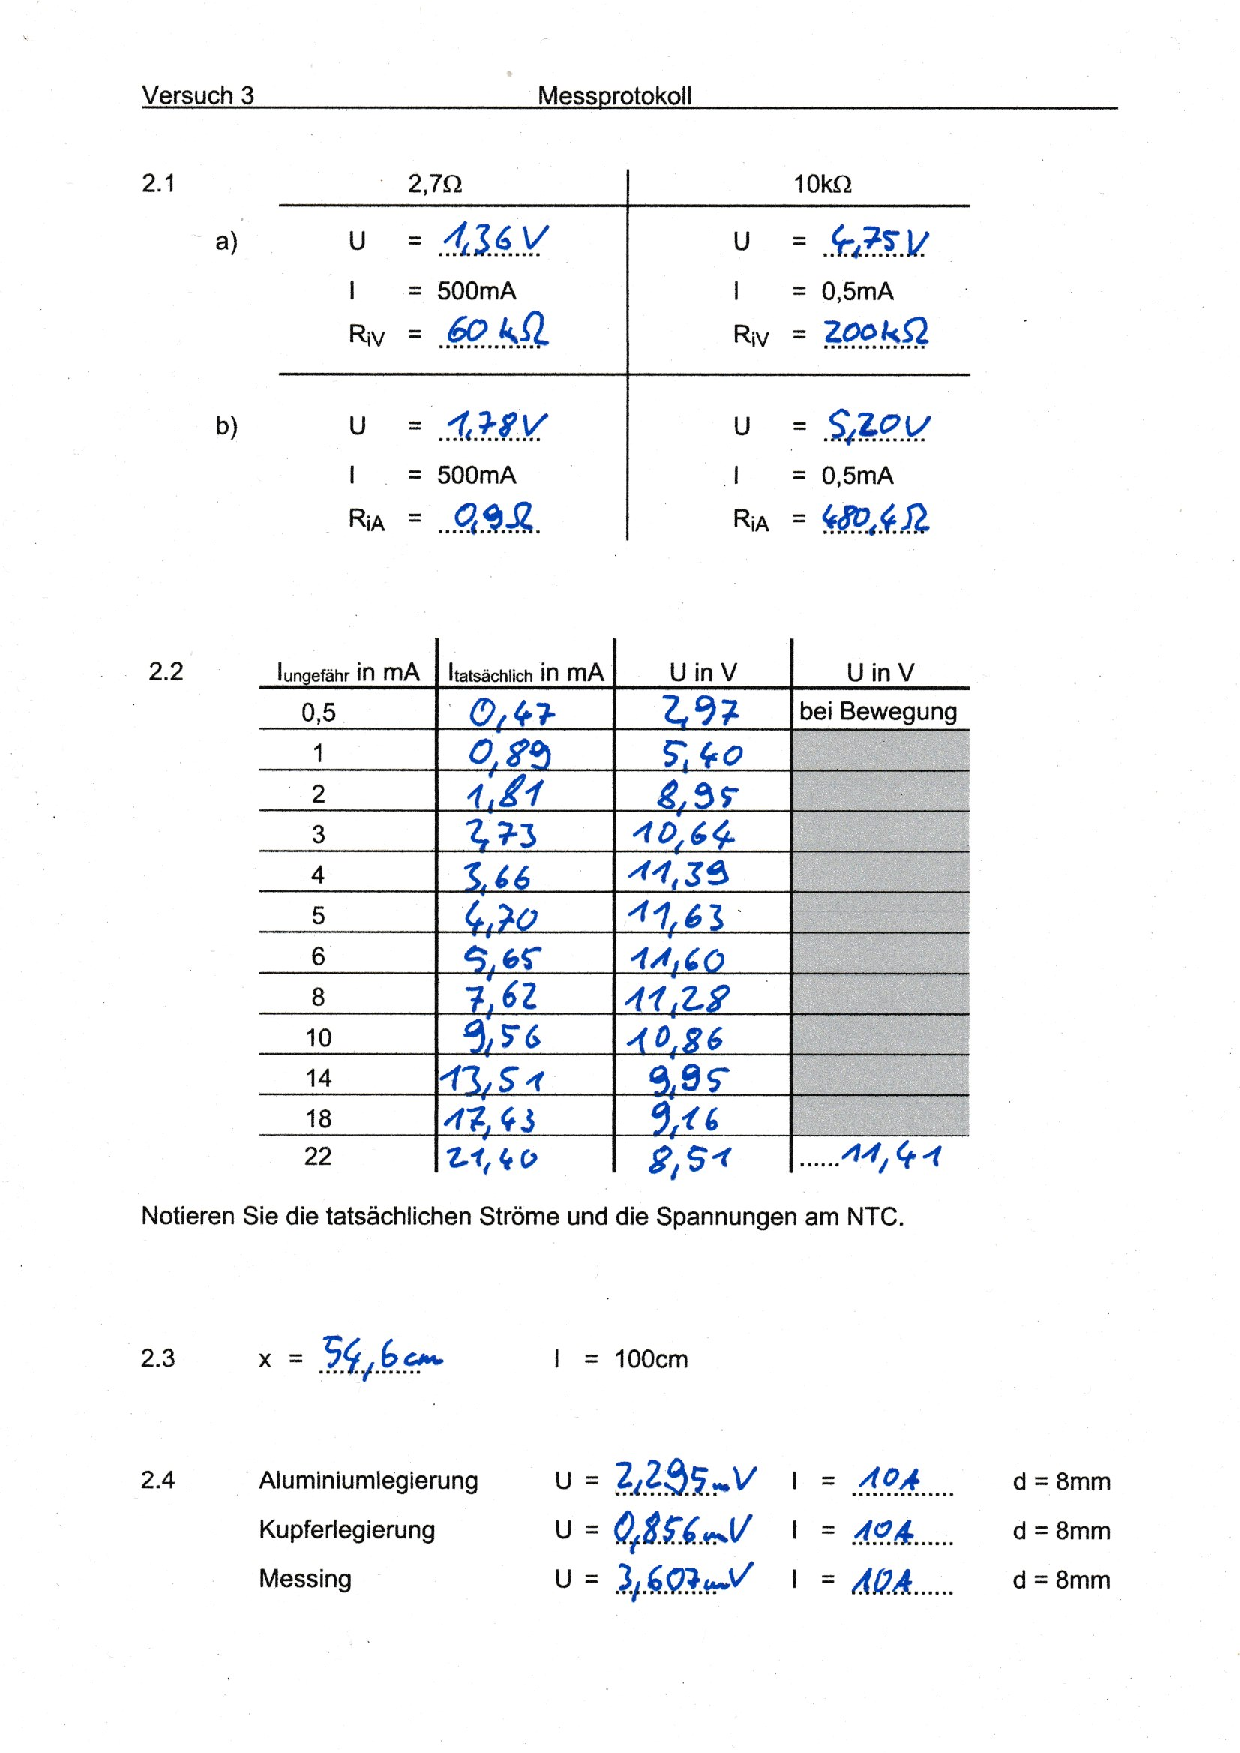
\includepdf[pages=-]{Messprotokoll.pdf}
\end{document}